\section{Experiments}
\label{sec:results}

\subsection{Experimental setup}
We evaluate Qwen2.5-Omni-7B and Qwen2.5-Omni-3B
\cite{qwen25omni2025}, alongside Fun-Audio-Chat-8B
\cite{funaudiochat2026}, on 600 shared synthetic soundscapes. Scaper
\cite{salamon2017scaper} combines single-label foreground recordings from
the FSD-MIX-SED source release \cite{wang2021shots}, derived from FSD50K
\cite{fonseca2021fsd50k}, with backgrounds from TUT Urban Acoustic Scenes
2018 \cite{heittola2018tut}. Each 10\,s recording sampled at 16\,kHz holds a
query event, a separate nuisance event, and continuous ambience at a nominal
$+10$\,dB event-to-background ratio. The evaluation covers 33 query classes
with event instances held out from the pilot. Two option orders yield 1,200
trials per condition and model. All three models exceed the protocol's 0.75
original-accuracy floor, and silence changes more than 20\% of answers.
Confidence intervals resample paired soundscapes, keeping both option orders
and all intervention conditions together.

\subsection{Class changes versus matched rewrites}
Different-class replacement changes the intended answer, while same-class
replacement rewrites the queried interval and preserves that answer.
Figure~\ref{fig:conditions} shows the resulting separation. The paired
answer-change gaps are 0.609, 0.578, and 0.497 for Qwen2.5-Omni-7B,
Qwen2.5-Omni-3B, and Fun-Audio-Chat-8B, respectively. Their 95\% intervals
in Table~\ref{tab:conditions} exclude zero. The independence reference in
Eq.~\ref{eq:independent-reference} is 0.538, 0.479, and 0.413. The observed
gaps exceed these values by 0.072, 0.099, and 0.084, which equal the
covariance corrections in Eq.~\ref{eq:dependence-correction}. The direction
holds across both model families and all 33 query classes. The smallest
class-level gaps are 3.8 percentage points for Fun-Audio-Chat-8B and 21.9
points for Qwen2.5-Omni-3B. The same-class response provides a reference for
answer changes caused by local waveform editing.

Figures~\ref{fig:class} and~\ref{fig:distribution} summarize the class-level
results. The scatter relates original recognition accuracy to the gap. The
cumulative curves display its distribution over all 33 query classes with
equal class weights. The positive class-level gaps show that the contrast
extends across all evaluated categories.

\begin{figure}[t]
\centering
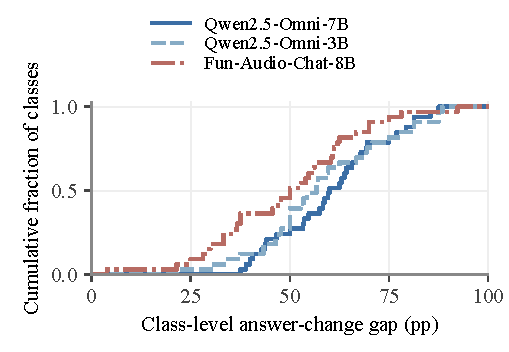
\includegraphics[width=\columnwidth]{figures/reference_distribution.pdf}
\caption{Empirical cumulative distributions of class-level answer-change gaps.
Each curve weights the 33 query classes equally and shows the fraction with a
gap at or below each threshold. Gaps are measured in percentage points.}
\label{fig:distribution}
\end{figure}

\subsection{Locality and editing controls}
Table~\ref{tab:conditions} reports the intervention profile. Nuisance removal
changes answers at rates of 0.055, 0.071, and 0.075 for the three models,
while background-window rates stay below 0.016 and sham rates below 0.010.
The much larger target response thus concentrates sensitivity on the queried
event, beyond the response to off-target edits or to the editing path alone.

\emph{Acoustic distance.} Among the 236 soundscapes, or 472 option-order
trials, with different-class and same-class log-mel edit distances matched
within 15\%, the trial-level gap is 0.617 for Qwen2.5-Omni-7B with a 95\%
interval of [0.555, 0.678]. For Qwen2.5-Omni-3B the gap is 0.530 with an
interval of [0.462, 0.597]. The corresponding full-set trial-level gaps are
0.609 and 0.578. Both matched-subset intervals exclude zero, supporting a
class-change interpretation at similar measured edit magnitudes.

\subsection{Selective accuracy on the replacement}
Table~\ref{tab:follow} complements answer changes with class recognition.
Same-class replacement retains accuracies of 0.859, 0.841, and 0.795 for
Qwen2.5-Omni-7B, Qwen2.5-Omni-3B, and Fun-Audio-Chat-8B, respectively,
compared with 0.882, 0.853, and 0.847 on the originals. Same-class accuracy
remains within 5.2 percentage points of original accuracy. The matched rewrite
therefore retains recognition performance close to the original. On eligible
trials, soundscape-weighted selective accuracy for the inserted class is 0.819, 0.801, and
0.737. On these trials, the correct different-class answer names the inserted
class. This directional measure distinguishes recognition of the replacement
from answer movement alone, as local class changes often lead models to identify
the newly inserted event.
